\clearpage

\section{Phase Mismatch Compensation}
\label{sec:phase_mismatch_compensation}
\begin{refsection}

\begin{tcolorbox}	
\begin{tabular}{p{2.75cm} p{0.2cm} p{10.5cm}} 	
\textbf{Header File}    &:& phase\_mismatch\_compensation\_*.h \\
\textbf{Source File}    &:& phase\_mismatch\_compensation\_*.cpp \\
\textbf{Version}        &:& 20190114 (Daniel Pereira)
\end{tabular}
\end{tcolorbox}

\subsection*{Input Parameters}

\begin{table}[H]
\centering
\begin{tabular}{|l|l|l|}
\hline
Name                         & Type           & Default Value \\ \hline
numberOfSamplesForEstimation & integer        & 21            \\ \hline
pilotRate                    & integer        & 2             \\ \hline
\end{tabular}
\end{table}


\subsection*{Methods}

\begin{itemize}
  \item PhaseMismatchCompensation(vector<Signal *> \&InputSig, vector<Signal *> \&OutputSig) :Block(InputSig, OutputSig)\{\};
  \item void initialize(void);
  \item bool runBlock(void);
  \item void setPilotRate(int pRate) \{ pilotRate = pRate; \};
  \item void setNumberOfSamplesForEstimation(int nSamplesEstimation) \{ numberOfSamplesForEstimation = nSamplesEstimation; samplesForEstimation.resize(nSamplesEstimation); \};
\end{itemize}




\subsection*{Input Signals}

\textbf{Number}: 1\\
\textbf{Type}: Complex (DiscreteTimeContinuousAmplitude)


\subsection*{Output Signals}

\textbf{Number}: 1\\
\textbf{Type}: Complex (DiscreteTimeContinuousAmplitude)

\subsection*{Functional Description}

This block accepts a complex constellation signal and outputs another complex constellation built from its input. The block assumes pilot-aided phase mismatch compensation is being performed, takes the pilot signals before and after each signal, makes an average of the phase in each pilot and uses that estimation to compensate the phase mismatch.

\subsection*{Theoretical Description}\label{bercalc}

The pilot-assisted phase mismatch compensation scheme employed in this block is based on the schemes proposed in~\cite{soh15,qi15}. A representation of the output of the modulation stage of a pilot-assisted \mbox{LLO CV-QC} scheme is presented in Figure~\ref{fig:pilotAssistedTimeDependence}. 
%
\begin{figure}[h]
\centering
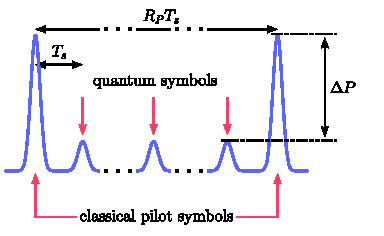
\includegraphics{./lib/phase_mismatch_compensation/figures/novelMethodTimeDependence.pdf}
\caption{Representative time dependence of a pilot assisted phase mismatch compensation signal.}
\label{fig:pilotAssistedTimeDependence}
\end{figure}
%
An unmodulated pilot signal is sent, time-multiplexed with the information carrying pulses, with the pilot signal being used to estimate the phase mismatch between the two lasers. At the receiver, the quantum and the pilot constellation are given, respectively, by
%
\begin{equation}\label{eq:signalAfterCoherentDetection} 
y_r(t_n)=
\begin{cases}
x_q(t_n)e^{i[\theta_q(t_n)+\epsilon(t_n)]},~n\neq mR_P \\
x_p(t_n)e^{i[\epsilon(t_n)]},~n=mR_P
\end{cases},~n,m\in\mathbb{N}.
\end{equation}
%
The phase mismatch for the nth pulse is estimated from an average of the phase of the previous and the later pilots, resulting in
\begin{equation}
\hat{\epsilon}(t_n)=\frac{\epsilon(t_{(m+1)R_P})+\epsilon(t_{mR_P})}{2},~mR_P<n<(m+1)R_P,
\end{equation}
with the mismatch compensation being accomplished by multiplying the constellation by $e^{-i(\hat{\epsilon}(t_n))}$, resulting in
\begin{equation}
x_q(t_n)e^{i[\theta_q(t_n)+\epsilon(t_n)-\hat{\epsilon}(t_n)]}.
\end{equation}


% bibliographic references for the section ----------------------------
\clearpage
\printbibliography[heading=subbibliography]
\end{refsection}
\addcontentsline{toc}{subsection}{Bibliography}
\cleardoublepage
% --------------------------------------------------------------------- 